\chapter{Novel Datasets for Transfer Learning}

\begin{remark}{Outline}

This chapter ...

\vspace{5mm}
\textit{This chapter is based on the publication \citet{sabatelli2021advances}.}
\label{ch:minerva_paper}


\end{remark}


\section{Challenges of Modern Computer Vision}
\label{sec:cv_challenges}


\subsection{Photo-realism}
\subsection{Data Scarcity}
\subsection{Irrelevant Training Categories}
\subsection{Model Robustness}



\section{The MINERVA Dataset}
\label{sec:minerva_dataset}

\subsection{Music Iconography}
\subsection{Data Collection}
\subsection{Annotation Process}
\subsection{Versions and Splits}

\begin{tabular}{l|rr|rr|rr} \hline
	$\mathcal{T}_T$ &  \multicolumn{2}{c}{training-set} & \multicolumn{2}{|c|}{validation-set} & \multicolumn{2}{c}{testing-set}\\
& $N_t$ & $I_t$ & $N_t$ & $I_t$ & $N_t$ & $I_t$ \\\hline \hline
\texttt{Minerva-0} & 1857 & 4243 & 1137 & 2288 & 1182 & 2102 \\
\texttt{Minerva-5} & 952 & 1589 & 540 & 852 & 721 & 1173\\
\texttt{Minerva-10} & 1227 & 2147  & 680 & 1127 & 897 & 1506 \\
\hline

\end{tabular}




\begin{figure}[htb!]
	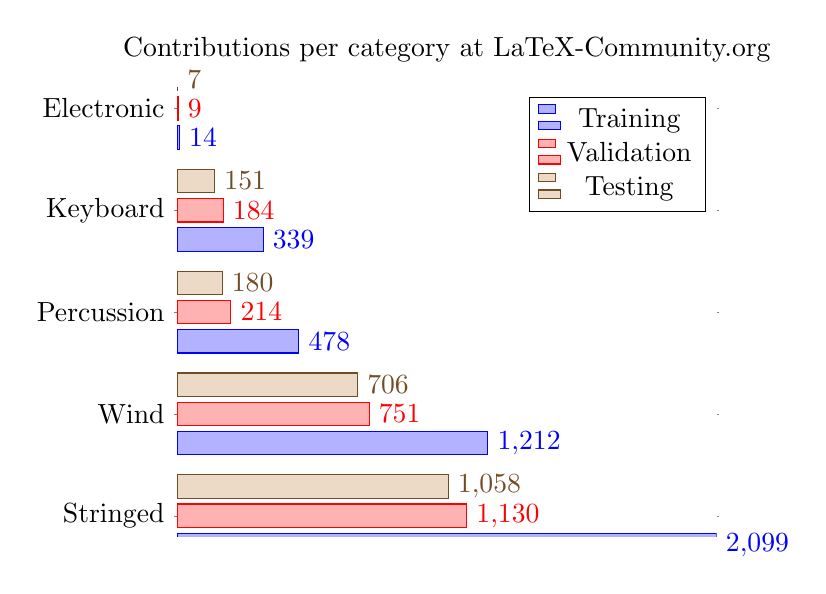
\begin{tikzpicture}
  \begin{axis}[title  = Contributions per category
                          at LaTeX-Community.org,
    xbar,
    bar width=.3cm,
    y axis line style = { opacity = 0 },
    axis x line       = none,
    tickwidth         = 1pt,
    enlarge y limits  = 0.05,
    enlarge x limits  = 0.001,
    symbolic y coords = {Stringed, Wind, Percussion,Keyboard, Electronic},
    nodes near coords,
  ]
\addplot coordinates {(2099,Stringed) (1212,Wind) (478,Percussion) (339,Keyboard) (14,Electronic)};
\addplot coordinates {(1130,Stringed) (751,Wind) (214,Percussion) (184,Keyboard) (9,Electronic)};
\addplot coordinates {(1058,Stringed) (706,Wind) (180,Percussion) (151,Keyboard) (7,Electronic)};
\legend{Training,Validation,Testing}

\end{axis}
\end{tikzpicture}

\iffalse
\end{axis}
\end{tikzpicture}
\fi

	\caption{}
	\label{fig:hypernym_distribution}
\end{figure}



\iffalse
\begin{figure}[htb!]
	%The matrix in numbers
%Horizontal target class
%Vertical output class
\def\myConfMat{{
{0.01,  30,  60,  10,  20,  30,  40,  50,  60,  60},  %row 1
{0.01,  30,  60,  10,  20,  30,  40,  50,  60,  60},  %row 2
{0.01,  30,  60,  10,  20,  30,  40,  50,  60,  60},  %row 3
{0.01,  30,  60,  10,  20,  30,  40,  50,  60,  20},  %row 4
{0.01,  30,  60,  10,  20,  30,  40,  50,  60,  20},  %row 5
{0.01,  30,  60,  10,  20,  30,  40,  50,  60,  20},  %row 6
{0.01,  30,  60,  10,  20,  30,  40,  50,  60,  20},  %row 7
{0.01,  30,  60,  10,  20,  30,  40,  5,  60,  20},  %row 8
{0.01,  30,  60,  10,  20,  30,  40,  50,  60, 20},  %row 9
{0.01,  30,  60,  10,  20,  30,  40,  50,  60,  20},  %row 10
}}

\def\classNames{{"A","B","C","D","E","F","G","H","I","J"}} %class names. Adapt at will

\def\numClasses{10} %number of classes. Could be automatic, but you can change it for tests.

\def\myScale{1.5} % 1.5 is a good scale. Values under 1 may need smaller fonts!
\begin{tikzpicture}[
    scale = \myScale,
    font={\scriptsize}, %for smaller scales, even \tiny may be useful
    ]

\tikzset{vertical label/.style={rotate=90,anchor=east}}   % usable styles for below
\tikzset{diagonal label/.style={rotate=45,anchor=north east}}

\foreach \y in {1,...,\numClasses} %loop vertical starting on top
{
    % Add class name on the left
    \node [anchor=east] at (0.4,-\y) {\pgfmathparse{\classNames[\y-1]}\pgfmathresult}; 
    
    \foreach \x in {1,...,\numClasses}  %loop horizontal starting on left
    {
%---- Start of automatic calculation of totSamples for the column ------------   
    \def\totSamples{0}
    \foreach \ll in {1,...,\numClasses}
    {
        \pgfmathparse{\myConfMat[\ll-1][\x-1]}   %fetch next element
        \xdef\totSamples{\totSamples+\pgfmathresult} %accumulate it with previous sum
        %must use \xdef fro global effect otherwise lost in foreach loop!
    }
    \pgfmathparse{\totSamples} \xdef\totSamples{\pgfmathresult}  % put the final sum in variable
%---- End of automatic calculation of totSamples ----------------
    
    \begin{scope}[shift={(\x,-\y)}]
        \def\mVal{\myConfMat[\y-1][\x-1]} % The value at index y,x (-1 because of zero indexing)
        \pgfmathtruncatemacro{\r}{\mVal}   %
        \pgfmathtruncatemacro{\p}{round(\r/\totSamples*100)}
        \coordinate (C) at (0,0);
        \ifthenelse{\p<50}{\def\txtcol{black}}{\def\txtcol{white}} %decide text color for contrast
        \node[
            draw,                 %draw lines
            text=\txtcol,         %text color (automatic for better contrast)
            align=center,         %align text inside cells (also for wrapping)
            fill=black!\p,        %intensity of fill (can change base color)
            minimum size=\myScale*10mm,    %cell size to fit the scale and integer dimensions (in cm)
            inner sep=0,          %remove all inner gaps to save space in small scales
            ] (C) {\r\\\p\%};     %text to put in cell (adapt at will)
        %Now if last vertical class add its label at the bottom
        \ifthenelse{\y=\numClasses}{
        \node [] at ($(C)-(0,0.75)$) % can use vertical or diagonal label as option
        {\pgfmathparse{\classNames[\x-1]}\pgfmathresult};}{}
    \end{scope}
    }
}
%Now add x and y labels on suitable coordinates
\coordinate (yaxis) at (-0.3,0.5-\numClasses/2);  %must adapt if class labels are wider!
\coordinate (xaxis) at (0.5+\numClasses/2, -\numClasses-1.25); %id. for non horizontal labels!
\node [vertical label] at (yaxis) {Output Class};
\node []               at (xaxis) {Target Class};
\end{tikzpicture}
}

	\caption{}
	\label{fig:hypernym_distribution}
\end{figure}
\fi



\section{Benchmarking}
\label{sec:benchmarking}

\subsection{Classification}
\subsection{Object Detection}


\iffalse
\begin{figure}[htb!]
	\scalebox{0.8}{\begin{minipage}{.5\textwidth}
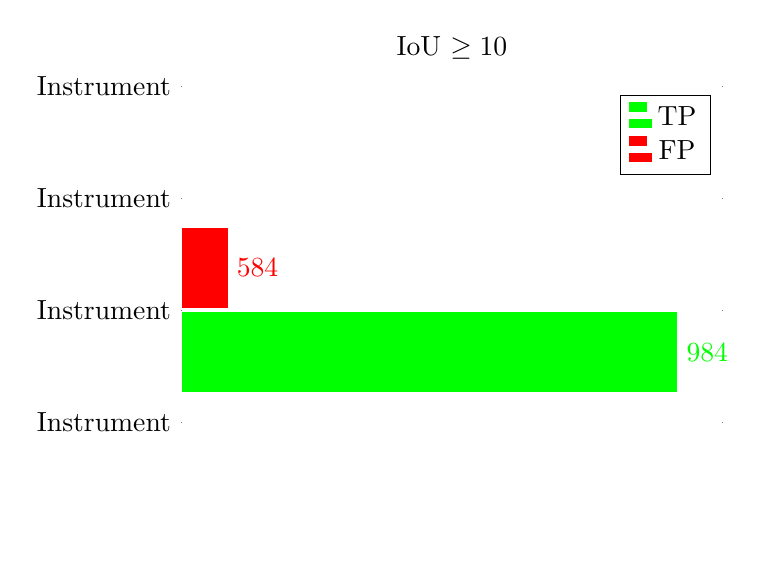
\begin{tikzpicture}
  \begin{axis}[title  = IoU $\geq 10$,
    xbar,
    bar width=1cm,
    y axis line style = { opacity = 0 },
    axis x line       = none,
    tickwidth         = 0.5pt,
    symbolic y coords = {Instrument},
    nodes near coords,
  ]
  \addplot [color=green,fill ] coordinates {(984,Instrument)};
  \addplot [color=red,fill] coordinates {(584,Instrument)};
\legend{TP,FP}
\end{axis}
\end{tikzpicture}
 \end{minipage}
 \hspace{3cm}
\begin{minipage}{.5\textwidth}
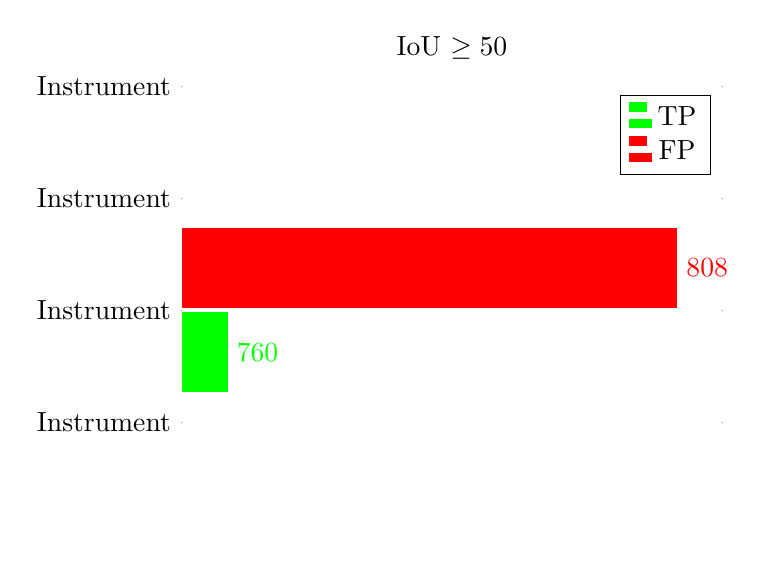
\begin{tikzpicture}
  \begin{axis}[title  = IoU $\geq 50$,
    xbar,
    bar width=1cm,
    y axis line style = { opacity = 0 },
    axis x line       = none,
    tickwidth         = 0.5pt,
    symbolic y coords = {Instrument},
    nodes near coords,
  ]
  \addplot [color=green,fill] coordinates {(760,Instrument)};
  \addplot [color=red,fill] coordinates {(808,Instrument)};
\legend{TP,FP}

\end{axis}
\end{tikzpicture}
 \end{minipage}
 

}
	\caption{}
	\label{fig:detection_experiment_1}
\end{figure}


\begin{figure}[htb!]
	\scalebox{0.8}{\begin{minipage}{.5\textwidth}
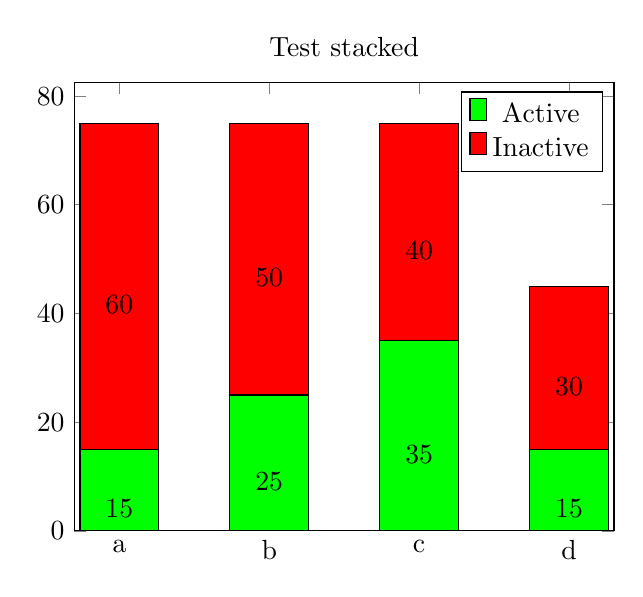
\begin{tikzpicture}
  \begin{axis}[
    title={Test stacked},
    ybar stacked, ymin=0,  
    bar width=10mm,
    symbolic x coords={a,b,c,d},
    xtick=data,
    nodes near coords, 
    nodes near coords align={anchor=north},%Move values in bar
    every node near coord/.style={
    },
  ]
  %Active
  \addplot [fill=green] coordinates {
({a},15)
({b},25)
({c},35)
({d},15)};
  %Inactive
  \addplot [fill=red] coordinates {
({a},60)
({b},50)
({c},40)
({d},30)};
  \legend{Active,Inactive}
  \end{axis}
 \end{tikzpicture}
 \end{minipage}
 \hspace{2.5cm}
\begin{minipage}{.5\textwidth}
 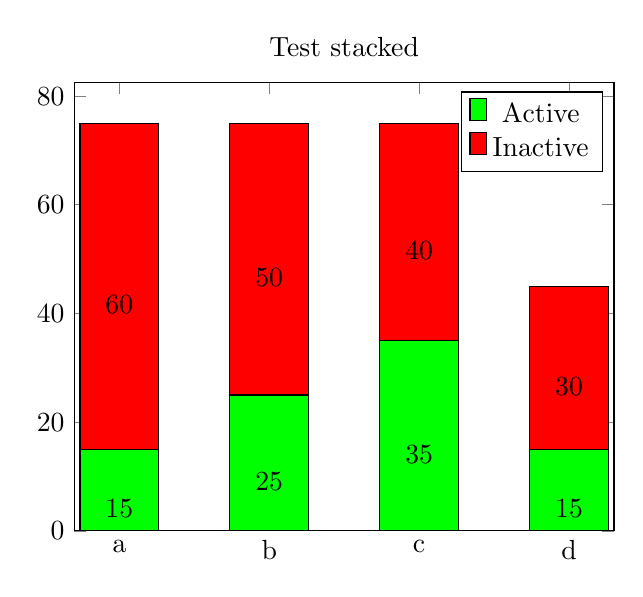
\begin{tikzpicture}
  \begin{axis}[
    title={Test stacked},
    ybar stacked, ymin=0,  
    bar width=10mm,
    symbolic x coords={a,b,c,d},
    xtick=data,
    nodes near coords, 
    nodes near coords align={anchor=north},%Move values in bar
    every node near coord/.style={
    },
  ]
  %Active
  \addplot [fill=green] coordinates {
({a},15)
({b},25)
({c},35)
({d},15)};
  %Inactive
  \addplot [fill=red] coordinates {
({a},60)
({b},50)
({c},40)
({d},30)};
  \legend{Active,Inactive}
  \end{axis}
 \end{tikzpicture}
 \end{minipage}

}
	\caption{}
	\label{fig:detection_experiment_2}
\end{figure}


\begin{figure}[htb!]
	\scalebox{0.8}{\begin{minipage}{.5\textwidth}
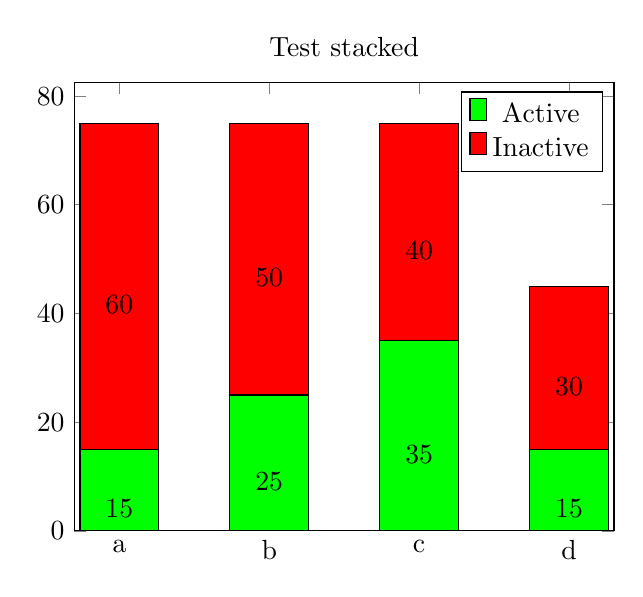
\begin{tikzpicture}
  \begin{axis}[
    title={Test stacked},
    ybar stacked, ymin=0,  
    bar width=10mm,
    symbolic x coords={a,b,c,d},
    xtick=data,
    nodes near coords, 
    nodes near coords align={anchor=north},%Move values in bar
    every node near coord/.style={
    },
  ]
  %Active
  \addplot [fill=green] coordinates {
({a},15)
({b},25)
({c},35)
({d},15)};
  %Inactive
  \addplot [fill=red] coordinates {
({a},60)
({b},50)
({c},40)
({d},30)};
  \legend{Active,Inactive}
  \end{axis}
 \end{tikzpicture}
 \end{minipage}
 \hspace{2.5cm}
\begin{minipage}{.5\textwidth}
 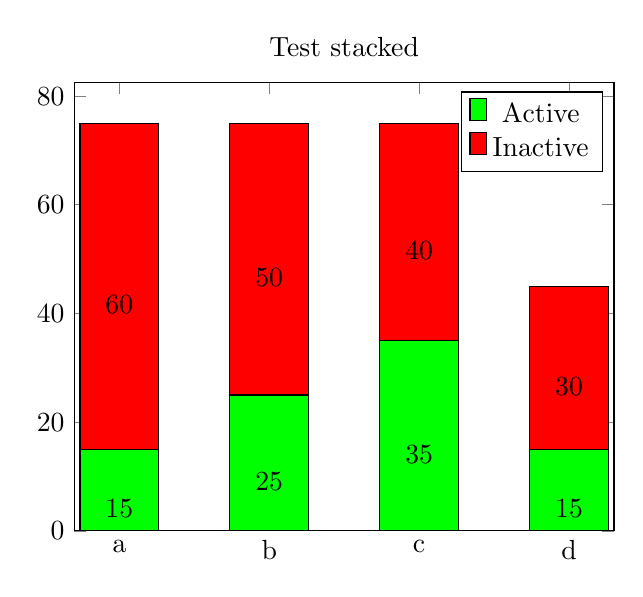
\begin{tikzpicture}
  \begin{axis}[
    title={Test stacked},
    ybar stacked, ymin=0,  
    bar width=10mm,
    symbolic x coords={a,b,c,d},
    xtick=data,
    nodes near coords, 
    nodes near coords align={anchor=north},%Move values in bar
    every node near coord/.style={
    },
  ]
  %Active
  \addplot [fill=green] coordinates {
({a},15)
({b},25)
({c},35)
({d},15)};
  %Inactive
  \addplot [fill=red] coordinates {
({a},60)
({b},50)
({c},40)
({d},30)};
  \legend{Active,Inactive}
  \end{axis}
 \end{tikzpicture}
 \end{minipage}

}
	\caption{}
	\label{fig:detection_experiment_4}
\end{figure}


\begin{figure}[htb!]
	\scalebox{0.8}{\begin{minipage}{.5\textwidth}
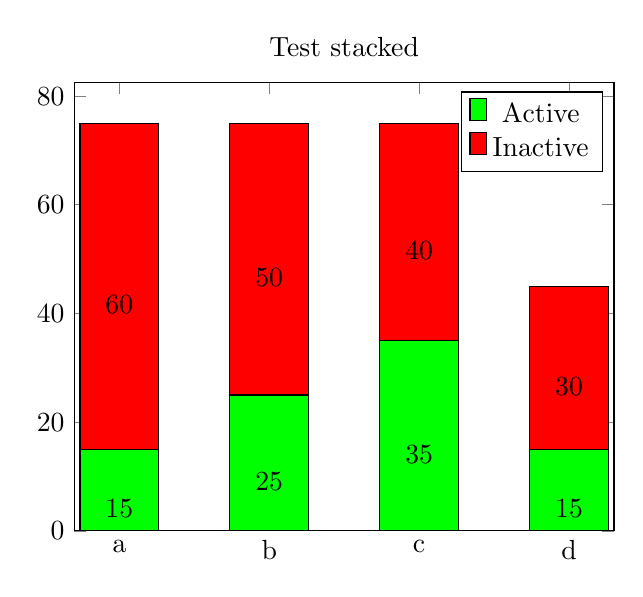
\begin{tikzpicture}
  \begin{axis}[
    title={Test stacked},
    ybar stacked, ymin=0,  
    bar width=10mm,
    symbolic x coords={a,b,c,d},
    xtick=data,
    nodes near coords, 
    nodes near coords align={anchor=north},%Move values in bar
    every node near coord/.style={
    },
  ]
  %Active
  \addplot [fill=green] coordinates {
({a},15)
({b},25)
({c},35)
({d},15)};
  %Inactive
  \addplot [fill=red] coordinates {
({a},60)
({b},50)
({c},40)
({d},30)};
  \legend{Active,Inactive}
  \end{axis}
 \end{tikzpicture}
 \end{minipage}
 \hspace{2.5cm}
\begin{minipage}{.5\textwidth}
 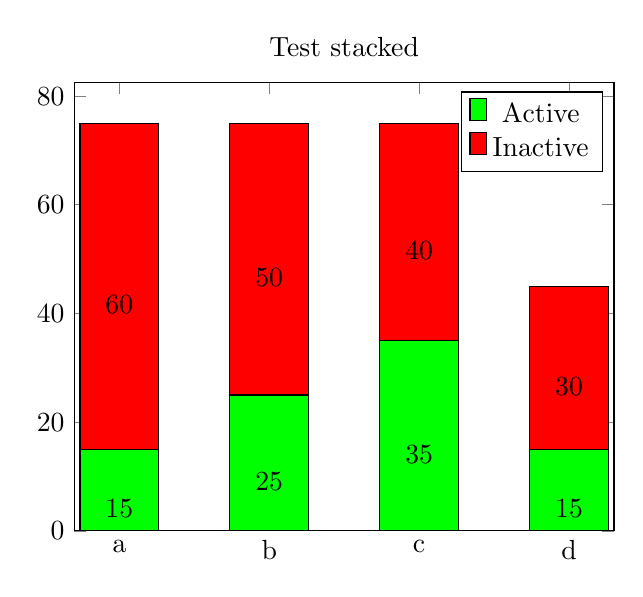
\begin{tikzpicture}
  \begin{axis}[
    title={Test stacked},
    ybar stacked, ymin=0,  
    bar width=10mm,
    symbolic x coords={a,b,c,d},
    xtick=data,
    nodes near coords, 
    nodes near coords align={anchor=north},%Move values in bar
    every node near coord/.style={
    },
  ]
  %Active
  \addplot [fill=green] coordinates {
({a},15)
({b},25)
({c},35)
({d},15)};
  %Inactive
  \addplot [fill=red] coordinates {
({a},60)
({b},50)
({c},40)
({d},30)};
  \legend{Active,Inactive}
  \end{axis}
 \end{tikzpicture}
 \end{minipage}

}
	\caption{}
	\label{fig:detection_experiment_4}
\end{figure}
\fi



\section{Results}
\label{sec:results}

\subsection{Quantitative Analysis}
\paragraph{Classification}
\paragraph{Object Detection}

\subsection{Qualitative Analysis}
\paragraph{True vs False Positives}
\paragraph{Saliency Maps}


\section{Discussion and Critical Analysis}
\label{sec:discussion}


\section{Future Work: towards more benchmarks}
\label{sec:future_work}
